\chapter{Implementation}
\label{chap:Impl}
\section{Programming APIs}

To implement VR applications, we can work directly with the SDK provided from each headset manufacturer, the advantage is that we can interact at a low level with the devices.\\ 
Another way is to use an SDK of a well-defined standard for example OpenVR from Valve or OpenXR from the Khronos group. This allows us to write applications for a target group of devices like 6-DOF supporting headsets without having to deal with different manufacturer SDKs (see Figure \ref{fig:openxr-overview}). On a side note: the X in OpenXR means that the specification is not only used for virtual reality (VR) applications but also for augmented reality (AR) and other technologies (XR) possibly proposed in the future.\\
Lastly, we can work with different engines which will provide with additional features. While classical desktop engines rely on downloading a complete bundled software package for distributing the application, WebXR and WebVR allow us to distribute and run our application via the browser, similar to WebGL.

At the time of writing, the OpenXR and WebXR specification is still relatively new being in its first revision therefore it is not implemented by each headset manufacturer, browser and engine yet. However, these standards are meant to replace the old OpenVR and WebVR in the future.

\begin{figure}[!hbt]
    \centering
    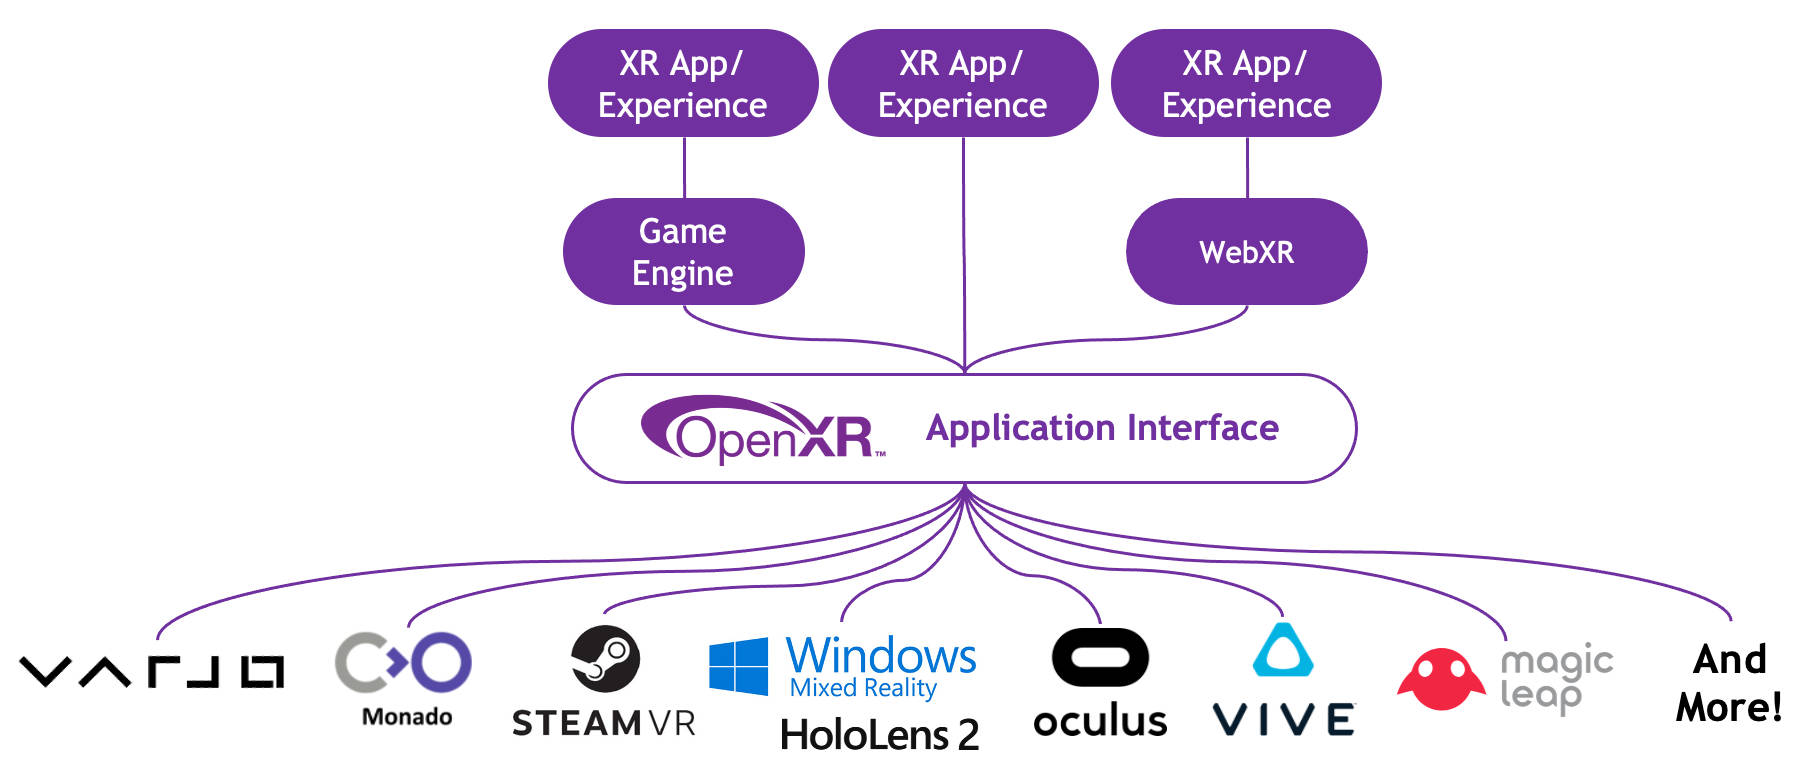
\includegraphics[width=\textwidth]{graphics/openXR-overview.jpg}
    \caption{Overview of the OpenXR API Stack \cite{khronosGroupOpenXR}}
    \label{fig:openxr-overview}
\end{figure}

\section{Prior Publication}
For our implementation we extend the code of a prior publication from Sorger et al. \cite{sorger_immersive_2019}. 
They implemented an immersive visualization for node-link graphs without hierarchical information. Their implementation already contains a common force-based layout, the laser-pointer ray casting technique to select objects, a free flying as well as animated teleport navigation method and lastly a code structure with an included render engine. A screenshot of their work is shown in Figure \ref{fig:priorPublication}.\\
We extended their implementation by adding the ability to visualization hierarchical networks as described in Section \ref{chap:proposed-Solution}. To achieve that we had to adapt the layout algorithm, add transparent rendering, adapt some visual rendering aspects, change the target position for the animated teleport, change the controller button mappings, implement the link filtering technique, add automatic/manual scaling of the virtual scene and automatic/manual adaption of the free flying speed.
This process is described in detail in Section \ref{sec:applOverview} and \ref{sec:applDetails}.

\begin{figure}[!hbt]
    \centering
    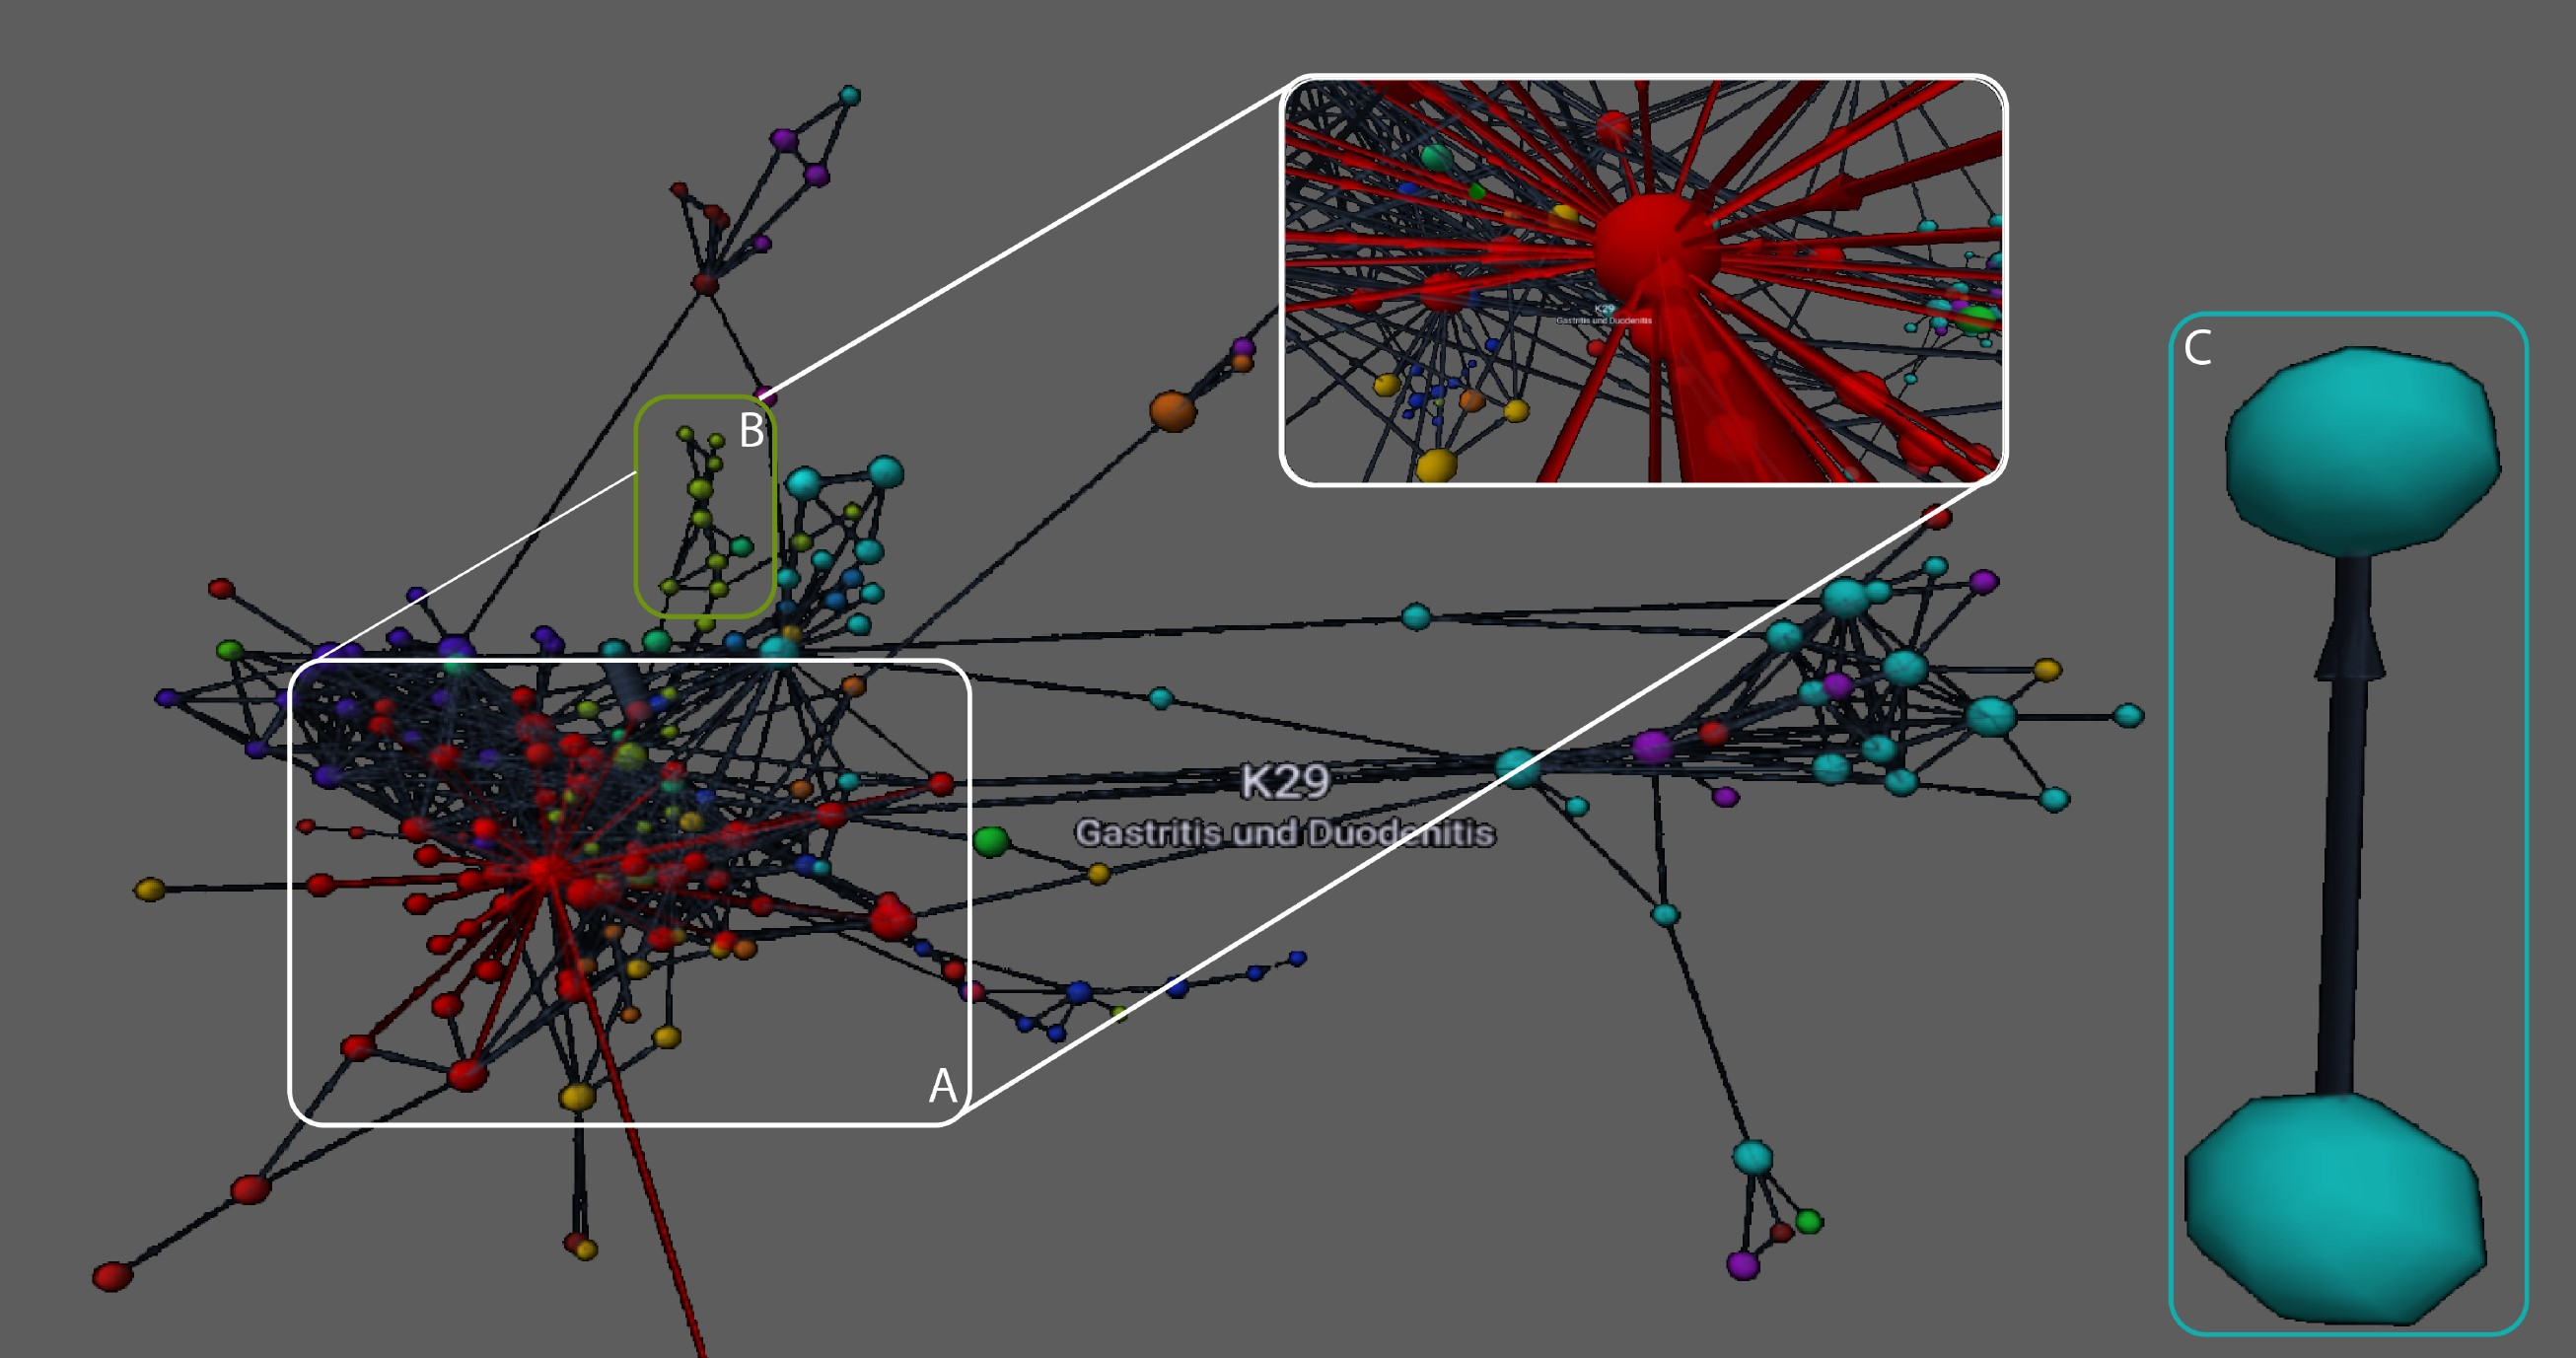
\includegraphics[width=\textwidth]{graphics/screenshotPriorPublication.jpg}
    \caption{Screenshot of the visualization from Sorger et al. \cite{sorger_immersive_2019} we extend our implementation on.}
    \label{fig:priorPublication}
\end{figure}

\section{Technology}

The application is implemented in plain JavaScript and runs in browsers that support the WebVR standard. 
At the time of writing this only applies to Firefox for Windows, our tested version is 85.0.2 (64-Bit). 
WebVR is already deprecated and being replaced with the new WebXR standard, therefore it is unlikely that other browser vendors will implement the standard in the future.\\
In order to reduce the complexity of the rendering and using the WebVR standard the application uses the framework A-Frame \cite{aframe}. A-Frame internally uses three.js \cite{threejs} as a render engine. The code from the publication we extended uses A-Frame in version 0.9.2 from September 2019, this version uses three.js version 0.108.0. 
The old version of A-Frame brings the limitation of only supporting WebVR because WebXR was not yet ready back in 2019. 
Updating A-Frame to a current version that supports WebXR was not possible within a reasonable time therefore we decided to stick to the old version and only support WebVR browsers and headsets.
The primary VR headset we are targeting with our application is the original HTC Vive.

\section{Application Overview}




\label{sec:applOverview}
\subsection{Data Structure}
\label{subSec:dataStruct}
To get a better understanding of the implementation we begin with the data structure for storing the graph.
Listing \ref{lst:internalJSON} shows a minimalistic example of the data structure that we use an input data source. The data is formatted as a JSON object with a flat list of nodes and link. The hierarchical information is encoded with the attributes childNodesIDs and parentNodeID as references. 
In addition to the necessary attributes, each node and link object can have additional attributes depending on the specific dataset.

\begin{lstlisting}[language=json,label={lst:internalJSON},caption=minimal JSON input data structure]
{
    "nodes": [
        {
            "id": "0.0",
            "weight": 4.5,
            "color": "rgb(77, 175, 74)",
            "layer": "0",
            "desc": "0.0",
            "childNodeIDs": [
                "1.1",
                "1.3",
                ...
            ]
        },
        ...
        {
            "id": "1.1",
            "weight": 1.7,
            "color": "rgb(250, 250, 110)",
            "layer": "1",
            "desc": "1.1",
            "parentNodeID": "0.0",
            "childNodeIDs": [
                "2.1",
                ...
            ]
        },
        ...
    ],
    "links": [
        {
            "color": "rgb(77, 175, 74)",
            "layer": "0",
            "source": "0.0",
            "target": "0.1",
            "label": "0.0 - 0.1",
            "linkwidth": 0.35
        },
        ...
    ]
}
\end{lstlisting}

\subsection{Program Flow}
\label{section:programFlow}
\begin{figure}[!hbt]
    \centering
    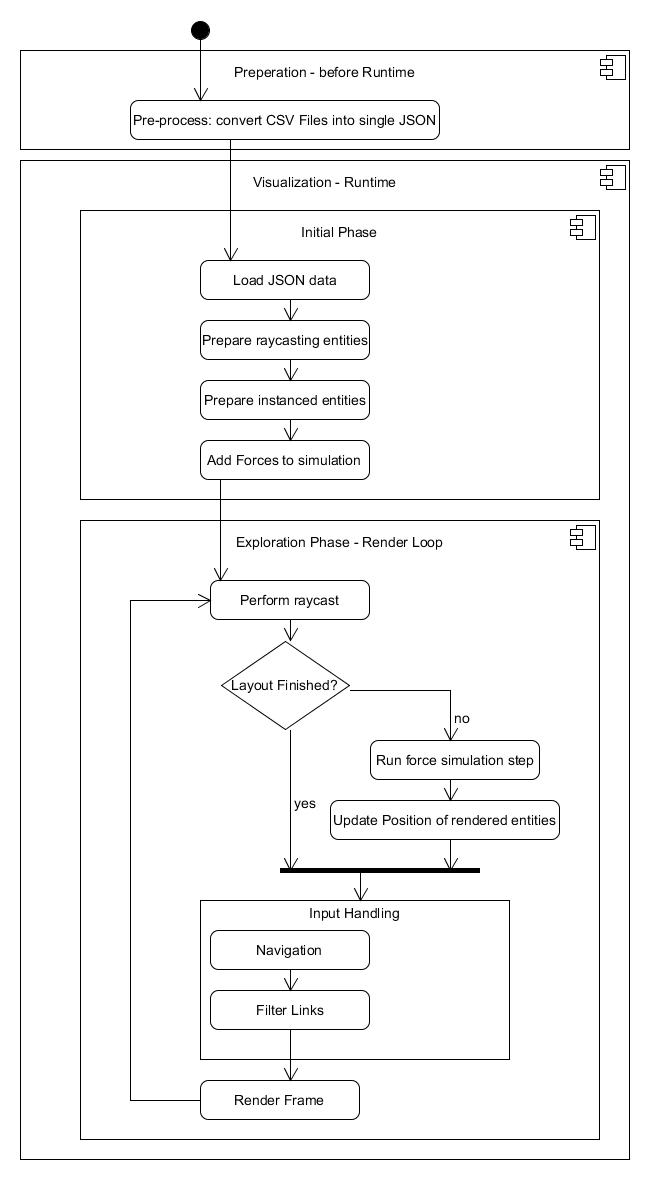
\includegraphics[width=0.74\textwidth]{graphics/vrgraph_flow.jpg}
    \caption{Sequence diagram of the program flow for our application.}
    \label{fig:impl_programFlow}
\end{figure}

We separated the application into multiple processing steps. Figure \ref{fig:impl_programFlow} describes the program flow and all abstract steps that are necessary for the visualization to work.
It contains of an offline preparation phase where the graph data is converted once to our internal JSON data structure (see Section \ref{sec:preprocessing}) and a runtime phase which is executed every time the browser loads the webpage.
After loading the data preparations for the instanced rendering (see Section \ref{sec:rendering}) and the force based layout (see Section \ref{sec:layoutCalculation}) are done.
Then the main render loop is executed which produces a rendered frame for each interaction. In addition, it handles the layout calculation (see Section \ref{sec:layoutCalculation}), navigation and interaction methods (see Section \ref{sec:vrInteractions}), scaling (see Section \ref{sec:scaling}), filtering the graph's links (see Section \ref{sec:linkFiltering}) and performing the ray casting for the virtual laser pointer.
The objects that got intersected by the virtual laser pointer are used in the navigation and interaction techniques. 
Details on how intersected objects are determined by ray casting is not further described as this method is already provided from the original implementation. 

\subsection{Virtual Scene Graph}
A-Frame application are build by creating a virtual scene graph.
It uses an entity-component-system architecture which follows the  composition over inheritance and hierarchy principle. 
This means that every object in A-Frame is an entity that can be customized by code.
There are various components that can be reused and extended, the base component is represented by the <a-entity> element.\\
Listing \ref{lst:virtualSceneGraph} shows a simplified version of the virtual scene graph the application uses. 
It consists of entities for both Vive controllers, a passive and active camera and rig setup and the graph object itself.
Most data and logic is encapsulated in the graphData object. We maintain here two lists of data: a list of nodes/links for the ray casting entities and a list of nodes/links for the actual rendered entities. 
The reason for this duplicated data is that we use  instanced objects for rendering (see Section \ref{sec:rendering}) and these can not be used for ray casting directly.

\begin{lstlisting}[label={lst:virtualSceneGraph},caption=Simplified virtual A-Frame scene graph used by the application.]
<body>
    <a-scene ... >
        <a-entity vive-controls="hand: left"> </a-entity>
        <a-entity vive-controls="hand: right"> </a-entity>
        
        <a-entity id="graphData" json-url="data/inputData.json" ... >
            <a-entity id="passive_rig"  ... >  
                <a-entity id="passive_cam" ... > </a-entity>
            </a-entity>
            ...
        </a-entity>

        <a-entity id="active_rig" ... >
            <a-text id="controllerLabel" ... > </a-text>
            <a-entity id="active_cam" ... > </a-entity>
        </a-entity>
        ...
    </a-scene>
</body>
\end{lstlisting}

\section{Application Details}
\label{sec:applDetails}
\subsection{Preprocessing Scripts}
\label{sec:preprocessing}

The visualization expects a combined JSON file with all nodes and links and their assigned layer as seen in Section \ref{subSec:dataStruct}.
A common data export format for networks are multiple CSV files, one file for the nodes and another for their edges.
In a hierarchical or clustered network there is an additional file with the hierarchical mapping.
Therefore, we needed a script to convert these CSV files to our JSON data format. For convenience most parameters can be configured by an additional config file without changing any program code. 
While transforming the data structure, all node IDs are extended with their hierarchical layer information to ensure unique IDs for the entire dataset.  
In addition, we also normalize the node and link width and add color attributes for a simplified rendering process later on.\\
To test our visualization with various networks of different sizes there is also a script for generating test data available.

\subsection{Layout calculation}
\label{sec:layoutCalculation}
Implementation Details of Forces, \\
Optimization for Saving Pos and set after done

\subsection{Rendering}
\label{sec:rendering}
Goal of Rendering: 
Performance, Support Transparency of nodes. 

Instancing per Links, 
Instancing per Hierarchical Layer of nodes, 
Transparency,
Wireframe

\subsection{VR Interactions}
\label{sec:vrInteractions}

Camera Rig vs Camera
camera rotation, correct position 
\\
extend controller
\\
Teleport => calculation of target Position (+Grafik?)
\\
FreeFly

\subsection{Scale}
\label{sec:scaling}

Move + Scale\\
Animation
\\

\subsection{LinkFiltering}
\label{sec:linkFiltering}

Filtering of Links\\
Algorithmus multilayer detail layout\\
